The Peersim implementation allowed us to test extensively the protocol under several conditions. The subsequent empirical analysis conducted proved Whanau to be resilient against malicious entities that could try to deny/delay access to the resources made available by the nodes. More importantly, it has shown to be resistant to clustering attack. In addition, the protocol does this in a completely distributed manner and without using external entities (e.g. central/third-party authorities). 

Thanks to the $w$-random walk sampling and the layered IDs, it manages to keep a fast one-hop \textsc{lookup} mechanism without compromising the Sybil-resistance property. It also succeeds to achieve this quality by keeping its routing table size to $O(\sqrt{mk}\log(km))$ (sublinear w.r.t. the network size $n$) entries per node.

Moreover, the majority of the bandwidth used globally by the protocol is utilised by the numerous random walks needed. These random walks just have to send $w=O(\log(n))$ messages each, thus leading to a small system load w.r.t the network size. This holds under the assumption of having few keys per node ($k=O(m)$ total keys, where $m$ is the number of honest edges), but also in the case of $k \gg m$.  Whanau would still be able to work using an acceptable share of network resources, without any major drawbacks.

There are however several ways in which we could improve our project and that are left to future works. We were not able to test it on real-world social network datasets, because mainly of experimental constraints (not enough powerful computing architectures). Moreover, the code itself could be vastly improved such to reduce memory usage and speed.

However, despite these limitations, it safe to conclude that Whanau is effective in different cases and scenarios, making it affordable and reliable for systems which need to be Sybil-proof.

\begin{figure}[t!]
    \centering
    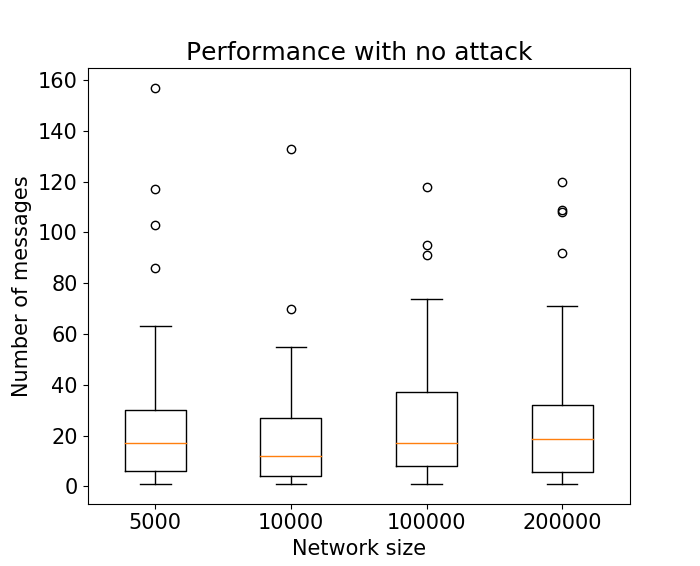
\includegraphics[scale=0.4]{exp3.png}
    \caption{Total number of messages sent by \textsc{lookup} procedure with a different network size $n$.}
    \label{fig:experiment_3}
\end{figure}